% ==============================================================================
% This file is part of the "LaTeX template for writing the Final Degree Work
% report". It has been developed to aid the students of the Bachelor's Degree in
% Video Game Design and Development at the Jaume I University.
%
% (c) 2019 Sergio Barrachina Mir and José Vte. Martí Avilés
%
% The template can be used and distributed under the next license:
%  Creative Commons Attribution-NonCommercial-ShareAlike (CC BY-NC-SA)
%  http://creativecommons.org/licenses/by-nc-sa/3.0/
%  http://creativecommons.org/licenses/by-nc-sa/3.0/legalcode
%
% Atom editor configuration follows:
% !TEX root = ./report.tex
% !TeX spellcheck = en-US
% ==============================================================================

\chapter{Work Development and Results}

\minitoc{}

\bigskip{}

In this section, we will detail the development of the project starting from the game creation, and then describing each step of increased complexity of the behaviour to imitate, as well as the results obtained in each step. 

To avoid confusion, we will refer to the programmed behaviors that we want to imitate as ``bot'' or ``NPC'', and the generated neural networks that have to learn to imitate that bot will be called ``AI'' or ``agent''.

\section{Game Development}

The game environment needs to include the ML Agents' classes (Agent and Academy) to train and play the game using the network. The game structure is the one shown in section~\ref{sec:system_design}.

The camera has an NPC and a trained AI attached: One of them controls its movement automatically, and who does that can be changed in play time. Both of these classes have getters to 3 variables that correspond to the possible movements: mouse X movement, mouse Y movement and mouse click, which are used to rotate and shoot.

The Spawner creates randomly and saves references of black planes in the scene, which correspond to the enemies.

To end with, a Debug Canvas has been added as interface, which draws lines with the movements made and the ones expected by the neural network. This allows to see how well the neural network is training.

\section{Reactive Behaviors}

The first human behavior we would analize is reactions, which can be defined as ``sudden changes produced by a stimulus''. To model this behavior, we created a Bot with the following requirements:

\begin{itemize}
 \item While not seeing any target, it moves to the left uniformly
 \item When a target enters the screen, it reacts moving fast towards its center, then continues moving as normal
\end{itemize}

At this first step, the bot will only move horizontally, and it will be considered that is always clicking (so the targets would be destroyed whenever the sight touches them).

\subsection{Training with Proximal Policy Optimization (PPO)}
\label{sec:trainingPPO}

Proximal Policy Optimization~\cite{ppopolicy} is the first and most simple reinforcement learning algorithm  provided by ML Agents~\cite{mlagents}. It uses a neural network to approximate the ideal function that maps an agent's observation to the best action it can take in a given state. Also, it is the fastest algorithm of all provided by ML Agents.

In the following subsections, some training related issues will be taken into account. At first, we will train our models using this policy (PPO).

\subsection{Unnecessary actions}
It is important not to add more actions than needed, since they would slow down the training process considerably. Even though it is possible to move in X and Y and perform clicks, since the bot only moves using the one axis, any additional action would add much noise to the AI. 

That is caused because when training the AI is overfitted with demonstrations with Y movements of exactly 0, and when that AI is playing any slight up or down movement would go inside untrained cases, and then causing unexpected behaviors.

Therefore, in this case the neural network would only have 1 action output: the X axis movement.

\subsection{Rewards based in tolerable range}
\label{sec:tolrange}

\begin{wrapfigure}{r}{0.35\textwidth}
    \centering
    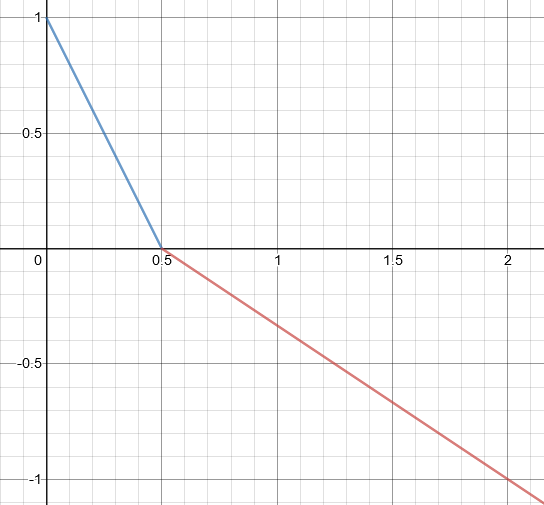
\includegraphics[width=0.35\textwidth]{img/rewTR.png}
		\caption{Rewards based in tolerable range.}
		\label{fig:trange}
\end{wrapfigure}

Our first reward approach is based in tolerable ranges. This consists in giving positive rewards when the distance between the guess and the real move is less than the tolerable range:

-The maximum reward is given (1) if it the distance is exactly 0

-A reward of -1 is given when the distance is 2, which is the maximum distance possible (NPC moving at maximum speed in one direction and the AI in the opposite direction).

In Figure~\ref{fig:trange}, you can see the reward function with tolerable range = 0.5. In our trainings, tolerable range was between 0.05 and 0.1: lower tolerable ranges than 0.05 caused the training to become unstable because it only got negative rewards, and higher tolerable range

Models trained using these rewards are not very time-efficient. If the tolerable range is too big (the agent receives positive rewards easily), the model doesn't fit the movement; if it is too small (receives negative rewards), the agent tends to stay only in the average movement, and doesn't react at all. That happens because the average is the point with biggest chance of reward (the agent is only punished when an impulse occurs). 

Curriculum learning~\footnote{Curriculum learning is a technique provided by ML Agents to train complex behaviors with consecutive lessons that increase in difficulty. That way, when the agent learns one task it goes on to the next lesson.} does not improve the training performance since with the initial less exigent punishments, the neural network learns much slower than with higher ones.

Figure~\ref{fig:graphTR} shows some of the success cases. From left to right, the first image shows how the neural network model adapts to the idle movement and the impulses, after 180000 training steps (4100s). The middle image displays an imperfect behavior of the same model when successive impulses occur. The right image is the same model trained longer time (10000s, 435000 steps), and how it tends to excessively smooth its impulsive movements. The causes of these two problems (successive impulses and smoothing) are discussed in section~\ref{sec:determ}.
\begin{figure}[h]
  \centering
		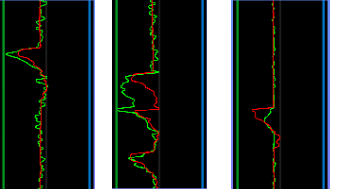
\includegraphics[width=.9\textwidth]{img/graphsTR.png}
  \caption{Bot movement (red) and neural network movement (green)}
  \label{fig:graphTR}
\end{figure}

\subsection{Determinism of the behavior}
\label{sec:determ}

Since at this point the neural network does not receive past events as input (neither moves or images), the movements performed by the bot have to be deterministic in order to train correctly: that is, given a frame, the bot would react with the exact same move every time (in the impulses, the default movement has a bit of noise in it). However, by how the bot was made it always took as objective the first image that it had seen, until destroyed.

In some special cases, when a new target spawns nearer to the sight than the current objective, the bot would not change the target order, and so it would behave differently depending on the context, as you can see in figure~\ref{fig:exDeterminism}. These repeated events cause the neural network to confuse when multiple targets are on screen, and if trained longer, it tends to do smaller impulses until only moving in the average move.

\begin{figure}[h]
  \centering
		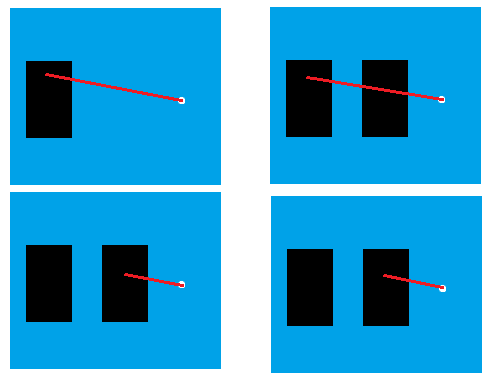
\includegraphics[width=.9\textwidth]{img/exampleDet.png}
  \caption{2 situations that lead to different actions with the same frame}
  \label{fig:exDeterminism}
\end{figure}

This issue is solved by making the bot behavior deterministic or adding a movement memory.

\subsection{Movement memory}
\label{sec:movememory}

In order to prepare the bot to have reaction times, 25 previous moves distributed in the last 2 seconds are added as observations. What move is added as observation is critical.

\begin{figure}[h]
  \centering
		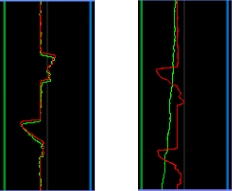
\includegraphics[width=.5\textwidth]{img/graphsMemory.png}
  \caption{A badly trained model while training (up) and playing (down)}
  \label{fig:graphMem}
\end{figure}

If the real bot movement is added, the bot reaches high rewards very quickly but doesn't learn to imitate the bot: that's because the neural network learns to ``mimic'' the last move made by the bot, so it has high chance of reward with only one important observation. When playing the game with the trained neural network, it would not move (in the beginning, all the previous moves are 0) until it starts moving in one or another direction at maximum speed (See Figure~\ref{fig:graphMem}). This happens when the movement starts increasing in value due to impressions in the returned action of the neural network that make it believe that it is accelerating in movement.

When using the neural network movement, it learns like before: correctly but a bit slower. However, the previous moves tend to have noise at first, and the network could learn to ignore them.

A better approximation would be interpolating the real move with the neural network's one: at the start, the movement added as observation in the next frames would be the NPC move. When the AI starts learning to adapt to the context (previous moves), the movement added would be an interpolation between the AI and the NPC movement (which would cause the AI to react in time), until the original AI moves are the ones added as observation. This can be made using curriculum learning: the lesson with least difficulty is the one where the AI receives past movements of the NPC as observations, and the hardest one where it receives its own movements as observation.

\subsection{Rewards based in standard deviation}
\label{sec:stdrew}

Since trained models using the methods explained in the previous sections tend to return the most common value, movements with more noise or imprecissions would not be produced correctly by the AI: when training, the AI could guess a move some units below the average of the previous moves but the NPC could have done a move the same units above the average, causing the network to be penalized, and causing the AI movement to converge to the average movement. To model these kind of noises more precisely, the actions and rewards should be changed.

In this section we propose a reward system based on standard deviations (Figure~\ref{fig:stdexample}): the relation between standard deviation, average and the actual move would determine how coherent is a move in a given context.
\begin{wrapfigure}{r}{0.2\textwidth}
    \centering
    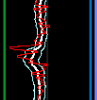
\includegraphics[width=0.2\textwidth]{img/graphSTD.png}
		\caption{Weighted average and standard deviations of an irregular movement}
		\label{fig:stdexample}
\end{wrapfigure}

The \emph{coherence} of a movement can be defined as how centered it is, in relation to the average. A movement with maximum coherence (1) would be the exact average, a movement at a standard deviation distance would have coherence 0, and movements outside of the standard deviations would be considered ``incoherent''. Then, default movement with noise would be coherent moves, and impulses would be incoherent.

To model the behavior, the agent would do 2 actions instead of one: a maximum and a minimum guess. The more precisely it encloses the real movement, the higher reward it gets; if it fails enclosing it, a punish is given.

\begin{figure}
    \centering
    \begin{subfigure}[b]{0.3\textwidth}
        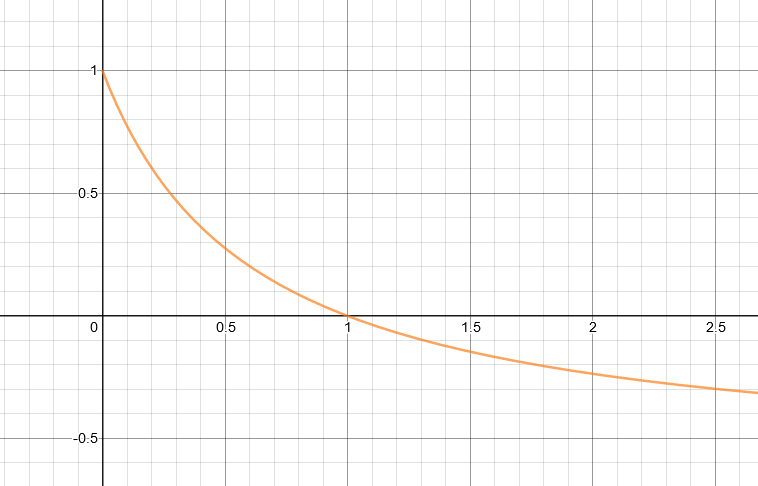
\includegraphics[width=\textwidth]{img/stdPrecision.png}
        \caption{Points by precision}
        \label{fig:prec}
    \end{subfigure}
    ~ %add desired spacing between images, e. g. ~, \quad, \qquad, \hfill etc. 
      %(or a blank line to force the subfigure onto a new line)
    \begin{subfigure}[b]{0.3\textwidth}
        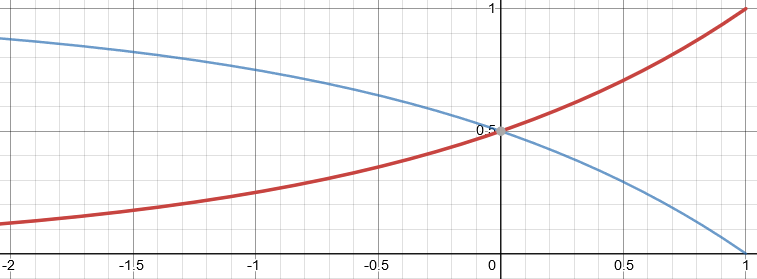
\includegraphics[width=\textwidth]{img/stdFactors.png}
        \caption{Reward and punishment factors by coherence}
        \label{fig:stdf}
    \end{subfigure}
    ~ %add desired spacing between images, e. g. ~, \quad, \qquad, \hfill etc. 
    %(or a blank line to force the subfigure onto a new line)
    \begin{subfigure}[b]{0.3\textwidth}
        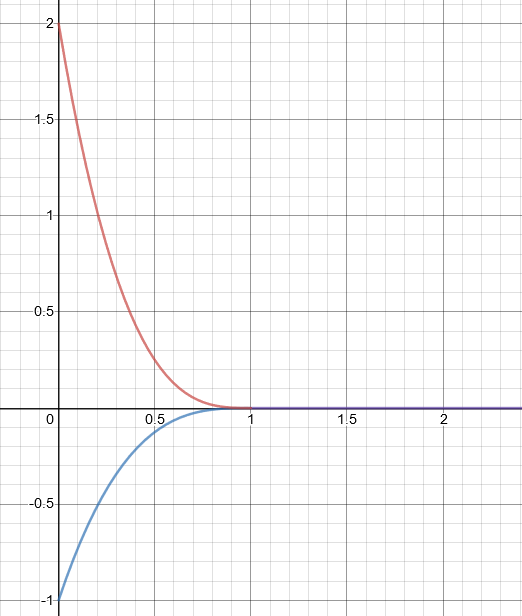
\includegraphics[width=\textwidth]{img/stdDevfactor.png}
        \caption{Deviation factor divided by Pow(2,(1-coherence)), with coherence=1}
        \label{fig:devf}
    \end{subfigure}
    \caption{Shape of the 3 parameters used for rewards}
		\label{fig:stdshapes}
\end{figure}

\begin{wrapfigure}{r}{0.2\textwidth}
    \centering
    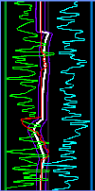
\includegraphics[width=0.2\textwidth]{img/graphsSTDrew.png}
		\caption{Trained model using SD rewards}
		\label{fig:stdrewards}
\end{wrapfigure}

Coherent moves give higher punishments if failing and smaller rewards, and incoherent moves (impulses) give high rewards. Given a maximum and minimum values (actions provided by the neural network), the real move, the average of the last 25 moves, its standard deviation and the coherence parameter explained in this section, the reward system follows these rules:

\begin{itemize}
 \item \emph{Coherence} is inversely proportional to the \emph{reward factor}, and directly proportional to the \emph{punish factor}: high coherence means lower rewards and higher punishes.
 \item A movement has higher \emph{precision} if it's centered between the maximum and minimum, and less if it's outside. The \emph{precision} is relative to the difference between the maximum and minimum values
 \item The \emph{deviation factor} is calculated dividing the real standard deviation with the agent one (max - min)
 \item The \emph{deviation factor} is inversely proportional to the coherence
 \item All the values are clamped to avoid excessively high rewards/punishments or zero division errors
 \item The final reward is calculated multiplying \emph{precision * factor * deviation factor}
\end{itemize}

In figure~\ref{fig:stdshapes} you can see the shapes of each parameter functions, used to calculate the final reward.


In this first approach using maximum and minimum estimations, the network doesn't fit well the movement: it encloses large areas continuously (See Figure~\ref{fig:stdrewards}). That could happen because it receives less punishment by enclosing the coherent movement than by fitting and sometimes failing, and also receives rewards from incoherent movement. Thus, the neural network finds an equilibrium enclosing wide ranges to catch high rewards from incoherent moves, at the cost of getting fewer rewards from coherent moves (which were low by definition) and not exposing to any punishment from failing to encase coherent moves.

\subsection{Rewards based in movement coherence}
\label{sec:cohrew}

Since last reward system didn't make the agent learn correctly, we need to change the rewards in a way that it worries about adjusting to the predictable coherent movement while also worrying about not to miss any impulsive incoherent move.

Rewards based on movement coherence are a simplification of the reward system exposed on section~\ref{sec:stdrew}, where coherent moves can only punish and incoherent moves can only give rewards. These motivates the agent to receive the least punishments by enclosing coherent moves, but also to take profit of potential rewards of incoherent moves. 

\begin{wrapfigure}[13]{rH}{0.4\textwidth}
    \centering
    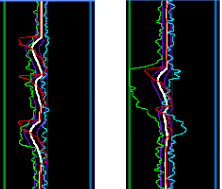
\includegraphics[width=0.4\textwidth]{img/graphsCoherence.png}
		\caption{Coherence-based models with and different learning rate: left=2e-3, right=8e-3}
		\label{fig:precisionR}
\end{wrapfigure}

The punishments in coherent moves are calculated multiplying the punish factor, the coherence (0..1) and the relative distance between standard deviations, maximum and minimum.

The rewards in incoherent moves are calculated using the reward factor, the opposite to coherence and the precision factor shown in section~\ref{sec:stdrew}.

Models trained with this system adapt better to both coherent and incoherent moves, however they need high learning rate and at least 300000 steps to see acceptable results (see Figure~\ref{fig:precisionR}). However, a learning rate higher~\footnote{Learning rate is an hyperparameter that defines the strength of each gradient descent update step} than 1e-2 can easily lead to unstable models that don't learn at all.

\subsection{PPO hyperparameters}

To sum up, the trained models that got decent performance had the following hyperparameters (they also depend on the reward system):

\begin{center}
	\begin{tabular}{ | m{4cm} | m{2.5cm}||m{4cm} | m{2.5cm} | } 
		\hline
			batch size & 32 or 1024 & beta & 5.0e-3..8.0e-3\\ 
		\hline
			buffer size & 256 or 8196 & epsilon & 0.3\\
		\hline
			hidden units & mostly 256 & learning rate & 1.0e-4..2.0e-3\\
		\hline
			learning rate schedule & mostly linear & normalize & false\\
		\hline
			num layers & mostly 1 & num epoch & 3-5\\
		\hline
			summary freq & 1000 & time horizon & 5-256\\
		\hline
			extrinsic strength & 1.0 & extrinsic gamma & 0.8..0.9\\
		\hline
			curiosity strength (opt.) & 0.01..0.1 & curiosity gamma (opt.) & 0.8..0.99\\
		\hline
			curiosity encoding size (opt.) & 128-256 & gail strength & 0.01 (not recommended)\\
		\hline
			gail gamma & 0.95 (not rec.) & gail learning rate & 0.0005 (not rec.)\\
		\hline
			gail encoding size & 64 (not rec.) & gail use vail & true (not rec.)\\
		\hline
			gail use actions & true (not rec.) & & \\
		\hline
	\end{tabular}
\end{center}

\subsection{Training with Soft-Actor Critic (SAC)}
\label{sec:trainingSAC}

Soft-Actor Critic~\cite{sacpolicy} is the second reinforcement learning policy provided in ML-Agents. It is characterized for being more sample-efficient and can learn from past experiences. However, it also executes slower, so the time needed to train a model is very similar both with PPO and SAC. Also, its training steps can be increased more easily since the learning rate is recommended to be constant (its Q function converges naturally).

To compare new methods with SAC and PPO, we've added simple linear rewards that affect the maximum and minimum individually, in addition to rewards based in movement coherence. These give reinforcement signals when one of the lines is well positioned, even when the cummulative reward is negative. In Figure~\ref{fig:pposac} you can see a cumulative reward comparison between an agent trained with SAC and other agent trained using PPO, with rewards based in coherence (see section~\ref{sec:cohrew}): SAC converges to a higher reward than PPO with much less steps.

\begin{figure}[h]
  \centering
		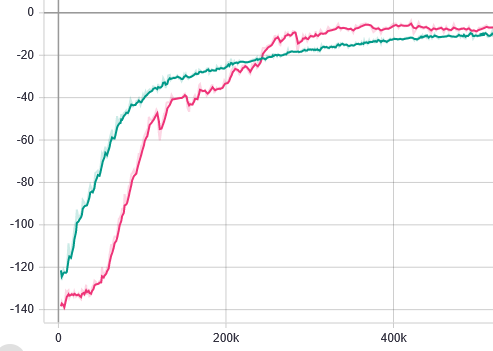
\includegraphics[width=.6\textwidth]{img/PpoSac.png}
  \caption{Total rewards of SAC (pink) and PPO (green).}
  \label{fig:pposac}
\end{figure}

As final result, Figure~\ref{fig:graphPS} shows a comparison between both trained neural networks: SAC adapts much better to impulses than PPO, even though PPO also manages to fit the real move between the two lines. However, when playing neither of them reacts correctly to targets that appear on the right side (mainly because it is an uncommon case). After the training both models still have much noise in their default movement, but it could be corrected by training longer or by rewarding the stability of both agent lines (maximum and minimum).

\begin{figure}[h]
  \centering
		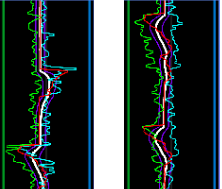
\includegraphics[width=.6\textwidth]{img/graphSacPpo.png}
  \caption{Comparison between SAC (left) and PPO (right).}
  \label{fig:graphPS}
\end{figure}

Another aspect to take into account is how both methods can be applied using GPUs to boost the training process. SAC makes better use of the GPU: by training with 3 environments in parallel the training speed doubles (being equally fast as PPO using CPU) and also improves its efficiency. PPO training using GPU and 3 environments is almost 2.5 times faster than with CPU or GPU-SAC, but is more likely to produce an application crash than any other training method (because of GPU overheating or running out of memory).

\subsection{SAC hyperparameters}

These parameters were the ones used when training with SAC:
\begin{center}
	\begin{tabular}{ | m{4cm} | m{2.5cm}||m{4cm} | m{2.5cm} | } 
		\hline
			batch size & 128 & buffer size & 200000\\ 
		\hline
			buffer init steps & 5000 & hidden units & 256\\
		\hline
			init entcoef & 1.0 & learning rate & 4.0e-4\\
		\hline
			learning rate schedule & constant & max steps & 6.0e5\\
		\hline
			memory size & 256 & normalize & true\\
		\hline
			num update & 1 & train interval & 5\\
		\hline
			num layers & 1 & time horizon & 64\\
		\hline
			sequence length & 128 & summary freq & 1000\\
		\hline
			tau & 0.005 & use recurrent & false\\
		\hline
			vis encode type & simple & pretraining strength & 0.4\\
		\hline
			pretraining steps & 20000 & extrinsic strength & 1.5\\
		\hline
			extrinsic gamma & 0.99 & curiosity strength & 0.03\\
		\hline
			curiosity gamma & 0.99 & curiosity encoding size & 128\\
		\hline
			gail strength & 0.03 & gail gamma & 0.99\\
		\hline
			gail encoding size & 128 & use actions & true\\
		\hline
	\end{tabular}
\end{center}

%-----------------------------------------------
%-----------------------------------------------
%-----------------------------------------------

\pagebreak

\section{Reaction time}

In this section we will cover the development of bots with a behavior similar to the one presented in last section, but with delayed reactions: when the bot sees a target, it does not react instantly, but takes a few milliseconds to perform the action. This adds more complexity to the behavior and to the neural network, since it needs to receive information from previous frames (Moreover, the reaction time may not be exactly the same every time).

Even though the AIs with actions based in standard deviation (2 outputs to encapsulate a noised movement, see~\ref{sec:stdrew}) did well modelling imprecise movements, we won't use this method in this section. That's because not only it would add more complexity to the task, but it could add much noise when moves are uncertain (if a bot reacts at 0.1-0.3 seconds, the AI would try to encapsulate a possible jump in all that range, and then if a random point in between was chosen as action each frame, the bot would not do a perfect impulsive movement. Instead, it would do a strange vibration). This feature will be solved with better reward systems (see section~\ref{sec:rtrewsys}).

\subsection{Render Textures}

In order to provide the agent past observations, render textures must be used (Camera observations aren't useful in this context since they cannot provide past frames as input). ML Agents allows to provide multiple visual inputs (see~\ref{fig:rendersens}), but they must follow these requirements:

\begin{itemize}
 \item Each render texture must have the same width and height~\footnote{This requirement also applies when only using one render texture (at least in this ML Agents version)}
 \item All render textures must be the same size
 \item All render textures must be either grayscale or not, but there must not be render textures of each type
 \item The minimum size is 20x20 pixels
 \item Each visual input must have an unique name (We use ``RenderTarget'' for the current frame and ``FrameXXX'' for past frames)
 \item Each visual input's render texture should not change in execution time~\footnote{Since there are multiple components of the same type, they cannot be changed reliably in real time}
\end{itemize}

\begin{figure}[h]
  \centering
		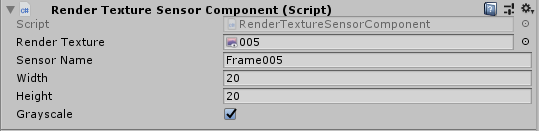
\includegraphics[width=.6\textwidth]{img/rendersensor.png}
  \caption{Example of a Render Sensor component.}
  \label{fig:rendersens}
\end{figure}

With these restrictions, there are two reasonable methods to manage render textures in Unity:

The first method consists in creating a Render Texture array with the desired frames in the N-1 position of the array (last frame in position 0, the 5th frame before in position 4...). The current frame isn't included in the array since it is rendered directly from a virtual camera. The missing positions in the array must be filled with other Render Textures, even though the neural network would not receive them as input. Then, when a frame ends each render target copies the next frame (iterating the array backwards), until the current frame is rendered over the render texture at the position 0.
This method is not very optimal and has some errors at the start (render textures appear empty until frame N, being N the size of the render textures array) but allows to personalize easily which frames we want to provide as input to the neural network. Also, sometimes the copying of frames can overlap (frame N is being drawn on frame N+1, but before ending the process the frame N-1 starts being drawn over frame N).

Other more optimal and safe~\footnote{Even though this method is safer, it is important to ensure that the render textures that won't be used again are deleted. Not doing so will cause the memory to overflow, and the environment to stop without apparent errors.} method is using a list to store previous frames like a queue (see Figure~\ref{fig:renderqueue} to visualize how it is executed): after each frame, a copy of the current rendered frame is saved at the start of the list, and the last is deleted if it exceeds the last frame provided as input. Then, for each frame that the network receives as input, the corresponding frame in the list is copied over it. With this method, each frame in the list isn't modified after being copied from the original.

\begin{figure}[h]
  \centering
		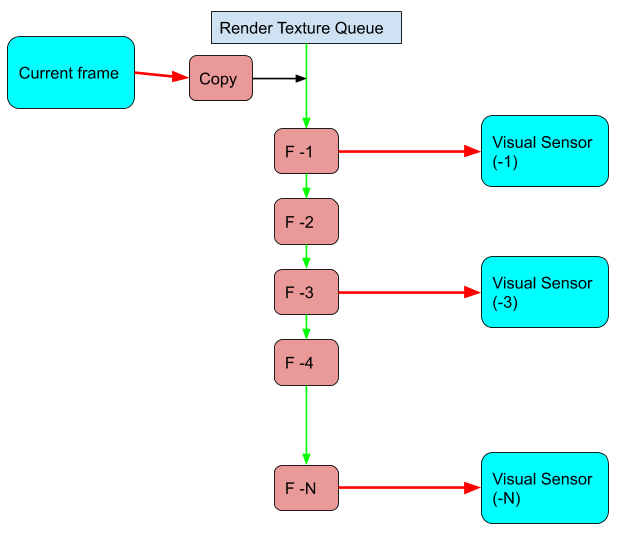
\includegraphics[width=.9\textwidth]{img/renderqueue.png}
  \caption{Render Queue: see that frame 2 isn't used as input for the neural network. Red arrows mean that the frame (or Render Texture) at the start is copied over the Render Texture at the end.}
  \label{fig:renderqueue}
\end{figure}

\subsection{Reward systems}
\label{sec:rtrewsys}

In this section, we've worked using 3 reward systems: tolerable range rewards, reward based in coherence and standard deviation and rewards after impulse.

\subsubsection{Tolerable range}

This reward system is the same that was described in section~\ref{sec:tolrange}. With delayed reactions, this system is only effective if they are uniform: all reactions must occur at the same time. If not, the neural network would consider that is not worth the risk of doing an impulse if that had high punishments (See Figure~\ref{fig:punDelay} to see an example of a high punishment when doing a correct impulse if the bot has non uniform reaction times).

With this method, the AI learned to do impulses correctly (even some that came from the right side, which is an exception case) but it didn't adapt well to the average movement: it had much more noise than the bot in default moves (See Figure~\ref{fig:timeTR}).

\begin{figure}[h]
  \centering
		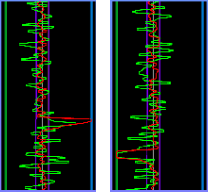
\includegraphics[width=.6\textwidth]{img/timeTR.png}
  \caption{AI trained with tolerable range rewards. It adapts well to the impulses but not so much to the normal movement.}
  \label{fig:timeTR}
\end{figure}

\subsubsection{Rewards after impulse}
\label{sec:afterimpulse}

This reward system uses 2 queues, one for the AI and other for the bot. Whenever one of them does an impulse, instead of giving a score to the moves, they are stored in a queue. Then, when the other one does another impulse it is compared with the first's movement (either the AI or the bot can do the impulse first). If one of them did an impulse but the other didn't, after some time the AI would be penalized (either by missing an impulse or by doing impulses when it shouldn't).

The results obtained using this reward system were not very good: the agents didn't learn to do impulses at all. Since the rewards are given after both impulses are completed, the AI can get confused about when to do an impulse and how~\footnote{It is important to use large (0.99-0.995) gamma values for the rewards in this method: a big gamma parameter means that the agent looks for future rewards.}. Even though, this method is still the easiest way to model temporal noise, and with better balanced rewards it should perform well (See Figure~\ref{fig:punDelay}).

\begin{figure}[h]
  \centering
		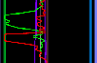
\includegraphics[width=.3\textwidth]{img/punDelay.png}
  \caption{Case when the AI would receive a double punishment when doing an impulse: if not using 2 queues, the agent would have a big punish even though the impulse was correct (the bot can react at either moment)}
  \label{fig:punDelay}
\end{figure}

\subsubsection{Rewards based in coherence and standard deviation}
\label{sec:rewchstd}

Like Tolerable Range rewards, this method has been applied to uniform reaction times. In our test cases, we have used reaction times between 1 and 8 frames of difference, and used as input for the AI the last 10 consecutive frames. This method is similar to the one explained in section~\ref{sec:cohrew}, but applied to one action instead of two (the expected move instead the maximum-minimum guesses).

This method differentiates between coherent and incoherent moves: when the bot's movement is coherent (it is inside the average$\pm$standard deviation range), the AI receives a consistent reward if its move is also inside that range, if not, it receives a punish that gets higher when the relative distance to that range increases. When the bot's movement is incoherent (impulse) there are 3 options:

\begin{wrapfigure}{rH}{0.2\textwidth}
    \centering
    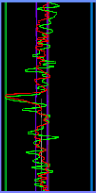
\includegraphics[width=0.2\textwidth]{img/graphRTstd.png}
		\caption{Model trained with 0.1 seconds of reaction time using this method}
		\label{fig:graphRTstd}
\end{wrapfigure}

\begin{itemize}
 \item If the AI move is closer to the bot's move than to the average, it receives a high reward (higher when closer)
 \item If the AI move is closer to the average move but between the average and the movement made, it doesn't receive any reward or punish
 \item If the AI move is in the opposite direction, it receives a punish
\end{itemize}

Using this method we have obtained the better results until this point (see Figure~\ref{fig:graphRTstd}), still, it has more problems imitating the exception cases (for example, when a target appears at the opposite side). 

The quality of this results is very dependent on the precision of the average and the standard deviation. In section~\ref{sec:dynamicstd} we explain how both of them were improved to get better results.

\subsubsection{Dynamic average and standard deviation}
\label{sec:dynamicstd}

At this point, to calculate the average and the standard deviation we were considering the last 60 moves. Each frame, the last move was deleted, the new one added to the list; then both the average and the standard deviation were updated. Using this amount of values was correct in some cases, but when some consecutive impulses happened they lost precision (see Figure~\ref{fig:stdVariations}), thus spoiling the reward system.

To add precision more values are needed, but too much values would be highly inefficient. To solve both of these problems, we use dynamic averages and dynamic standard deviations. Dynamic parameters are calculated using available previous information to avoid recalculating both values each frame: instead, when adding a new value, we use the last average (and standard deviation) and incorporate the new value to obtain the new average (or standard deviation). Both of them have O(1) computational cost (each frame) instead of O(N).

The dynamic average formula is the following:

\vspace{5mm}

$ {\displaystyle a_{n+1}=\frac{x_{n+1}+n\cdot a_n}{n+1}} $\\\\

Where we obtain the average for the next frame ($a_{n+1}$) from the last average ($a_{n}$), the new move value ($x_{n+1}$) and the amount of moves that have been used to calculate $a_{n}$ (n). Even though the formula can be obtained intuitively, the calculations used are explained at Appendix~\ref{app:average}.

\vspace{5mm}

The calculations needed to obtain the standard deviation $\sigma_{n+1}$ of the next frame require the last standard deviation $\sigma_{n}$, the new and old averages ($a_{n}$, $a_{n+1}$), the new move value ($x_{n+1}$), the amount of moves (n), and the average of all the moves squared ($\frac{\sum_{i=1}^{n}x_i^2}{n}$). This last parameter can be easily tracked using the dynamic averages explained above. 

The formula (see Appendix~\ref{app:stddyn}) for the dynamic standard deviation~\footnote{In the formula, the variance is used instead of the standard deviation to simplify the calculations, but we use only the standard deviation value} is the following:

\vspace{5mm}

$ {\displaystyle v_{n+1} = v_n + a_n^2-a_{n+1}^2 - \frac{\frac{\sum_{i=1}^{n}x_i^2}{n} - x_{n+1}^2}{n+1} } $\\\\

\noindent
The standard deviation is obtained taking the square root of the variance (v): $\sigma_n=\sqrt{v_n}$

Even though these two formulas stabilize both values, the standard deviation fails enclosing the noise of the coherent movement (it should be smaller) when there is a relatively big amount of impulses. To adapt better to the coherent movement, we interpolate the values of the moves outside of the standard deviation range~\footnote{Smoothing values may not be statistically correct for a standard deviation, but since the objective is to differentiate between Coherent and incoherent moves it is valid for our purpose}. From several training sessions, the best interpolation parameter for the real move and its closer standard deviation appears to be 0.4 (0.4·move + 0.6·standard deviation). Smaller interpolation parameters still made the range too big, and bigger interpolation parameters caused the standard deviation to increase too slowly~\footnote{The ideal interpolation parameter is approximately 0.4, however other parameters could work better with different amounts of noise. Still, this value works well in most of the cases.} (a parameter of 1 would cause the standard deviation to stay at value 0). See Figure~\ref{fig:stdVariations} to view a comparation between smoothed dynamic standard deviation, pure dynamic standard deviation and the non dynamic one.

\begin{figure}[h]
  \centering
		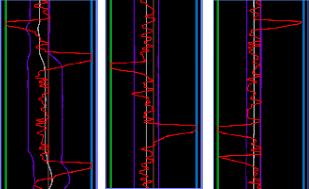
\includegraphics[width=.6\textwidth]{img/stdVariations.png}
  \caption{Standard variations and average of the same bot using last 60 values (left), dynamic values (mid) and dynamic values smoothed by a 0.6 interpolation (right)}
  \label{fig:stdVariations}
\end{figure}

\subsection{PPO vs. SAC}

As we said in section~\ref{sec:rewchstd}, it is possible to model a correct behavior using a reward system based in standard deviations and movement coherence. However, it is important to clarify that all of those good results were obtained using PPO.

Even though SAC was more effective modeling non delayed reactive behaviors (see~\ref{sec:trainingSAC}), PPO performed better with delayed reactions. This could be caused because how both algorithms work and because unbalanced rewards:

PPO tends to optimize the agent to have the highest rewards in each situation, but SAC optimizes it to have an overall higher reward. Agents trained with SAC tend to the average move, not doing any impulse. PPO follows the impulses since approaching them gives a potentially higher reward in that situation. Still, SAC models had better scores just by not exposing themselves to the punishments of failing coherent moves (which were higher than the punishments of failing an impulse). In Figure~\ref{fig:rtsacppo} you can see a comparison between both methods using the same reward conditions.

\begin{figure}[h]
  \centering
		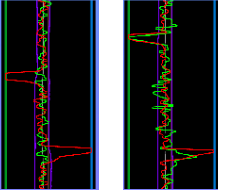
\includegraphics[width=.6\textwidth]{img/rtSACvsPPO.png}
  \caption{Comparison between an agent trained with SAC (left) and other trained using PPO (right). The bots in both cases have a reaction time of 0.1 seconds and 0.15 units of noise}
  \label{fig:rtsacppo}
\end{figure}

At this point, even though PPO performs better, both methods still fail at performing some impulses, when targets appear at the right side, or when two consecutive targets appear at the same time, and they don't adapt to noised reaction times (at least with the reward system exposed until this section).

\subsection{Behavioral cloning}
\label{sec:timeBC}

\begin{wrapfigure}{rH}{0.3\textwidth}
    \centering
    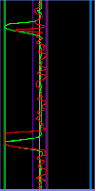
\includegraphics[width=0.2\textwidth]{img/bcTNoise.png}
		\caption{Model trained with BC in 2000 steps. The bot's impulses appear deformed because the agent is the one playing the game}
		\label{fig:bcTNoise}
\end{wrapfigure}


Behavioral Cloning~\cite{Sammut2010} is the simplest algorithm provided by ML Agents in terms of difficulty to adjust: it directly copies the actions given in a demo (which can be recorded in the editor). However, it has its limitations: since it doesn't depend on environment rewards, the programmer cannot modify its behavior with reinforcement learning. Also, depending on the task, agents trained using these methods can have chaotic behaviors.

\begin{wrapfigure}[17]{rH}{0.3\textwidth}
    \centering
    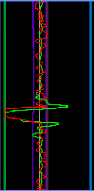
\includegraphics[width=0.2\textwidth]{img/bcTNovertrain.png}
		\caption{Model trained with BC in 7000 steps}
		\label{fig:bcTNovertrain}
\end{wrapfigure}

When trained with simple cases (in section~\ref{sec:spawner}, we treat how the rare cases were suppressed from the training), they perform really well. Also, the agents can model temporal noise effectively. The agent in Figure~\ref{fig:bcTNoise} is a simple case at the extreme: it receives the last 9 frames (and the current) as input and the bot can perform an impulse at each one of those frames (from 0.01s to 0.15s). The agent usually does the impulse at the average reaction time of the bot. It is worth noting that when the agent performs more or less correctly it's better to stop training, else it usually loses precision (see Figure~\ref{fig:bcTNovertrain}).

In the next 3 subsections, we will explain some problems that appeared when using behavioral cloning, and how they were solved.

\subsection{Recurrent memory} %lo de que se desvia por el input

Recurrent neural network~\cite{zaremba2014recurrent} are a feature that allow agents to have memory and remember past observations. They have the advantage of being optimized to ``choose'' what to remember, at the cost of giving less control to the user. Also, its training is much slower, and they have worse performance when infering.

A combination of past render targets, past moves and recurrent memory can obtain good models (even in some rare cases), but the resulting neural network is so heavy that the frame rate drops from roughly 70 fps to 25 fps. Even though it can perform most of the impulses, it usually has some strange artifacts (extra impulses) in its behavior (See Figure~\ref{fig:recb}).

One problem~\footnote{According to the ML Agents documentation, recurrent memory is not recommended for continuous action spaces, which we are using} that appears when using recurrent networks with simpler inputs is that they are not foolproof: whenever they receive an unexpected input (in most of its inputs), its behavior can become chaotic. In figure~\ref{fig:recc} you can see an example of this problem: the neural network appeared to have trained well, but when it received an empty input for the past moves (at the start, all previous moves are 0), when they were returned by the recurrent memory, the agent became chaotic.

\begin{figure}[h]
    \centering
    \begin{subfigure}[h]{0.3\textwidth}
        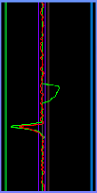
\includegraphics[width=\textwidth]{img/recurrentBrute.png}
        \caption{20 visual inputs and 25 past moves}
        \label{fig:recb}
    \end{subfigure}
    ~ %add desired spacing between images, e. g. ~, \quad, \qquad, \hfill etc. 
      %(or a blank line to force the subfigure onto a new line)
    \begin{subfigure}[h]{0.3\textwidth}
        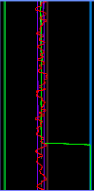
\includegraphics[width=\textwidth]{img/recurrentCaos.png}
        \caption{1 visual input and 25 past moves}
        \label{fig:recc}
    \end{subfigure}
		\caption{Agents trained with recurrent memory and behavioral cloning}
\end{figure}

In conclusion, recurrent neural networks are not recommended for this problem: behavioral cloning can adapt to the movement without them, and the training sessions and performance become much slower.

\subsection{Rare situations} %spawner
\label{sec:spawner}

As the game was programmed, targets spawn randomly at the stage. Since they can appear at any point, this provokes some situations that happen rarely: for instance, with the bots we have been using most targets appear by entering the screen in the left side (the bot moves continuously in that direction). However, some targets can spawn at its right side in a way that they can be seen, this happens approximately 1 in 12 times (the bot has a field of view of almost 60º). In figure~\ref{fig:spawncases} you can see some examples of some types of situations that appear in game.

\begin{figure}[h]
  \centering
		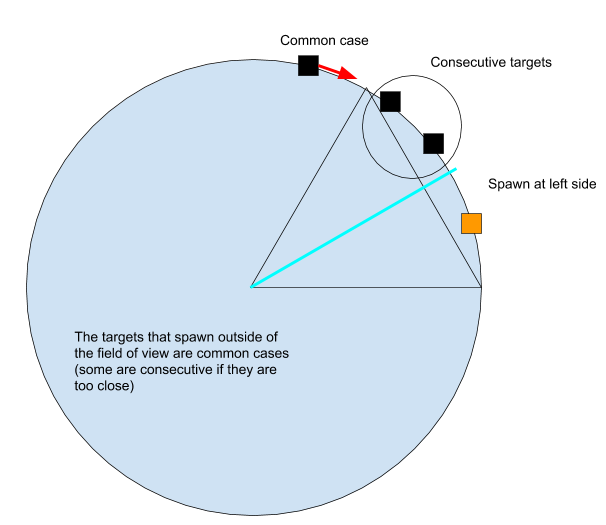
\includegraphics[width=.6\textwidth]{img/spawncases.png}
  \caption{Some of the different situations the neural network can encounter in the game}
  \label{fig:spawncases}
\end{figure}

Those rarer cases often suppose a harder task to solve by the neural network, but with temporal delays sometimes they cause the problem to be too complex to be approximated by the neural network (see Section~\ref{sec:complex}). Also, when they appear less times, they are learned slowly or not at all.

To improve the performance of the network, we can generate some rare cases in purpose: instead of spawning targets randomly, they can be spawned in the right side of the field of view, or two targets can be spawned next to each other, etc. Then, how often each case occurs can be adjusted manually.

\begin{wrapfigure}[9]{rH}{0.25\textwidth}
    \centering
    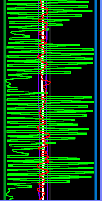
\includegraphics[width=0.2\textwidth]{img/complexity.png}
		\caption{Neural network that has diverged}
		\label{fig:complexity}
\end{wrapfigure}

This method was intended to make the agents learn faster, however it served to prove that the structure of the neural network was not enough to solve this problem.

\subsection{Complexity of the task} 
\label{sec:complex}

Sometimes a task is too complex to solve by one neural network structure, with behavioral cloning is easy to detect this problem~\cite{xor}. These problems need more internal layers (and more training time) to be solved. For instance, the problem developed in this section (delayed reactions) needed at least 3 layers (with any policy) to be solved. When spawning rare cases more often, some agents that usually didn't learn the exceptions didn't also learn the common cases: the complexity to perform correctly each case was too high for 3 layers.


When using behavioral cloning this phenomenon occurs like this: the neural network starts adapting to the most common cases (but fails the least common), then the more time it is left training, the worse starts doing the common cases until the model diverges (Figure~\ref{fig:complexity}) and it starts showing strange behaviors. Sometimes it may cycle around all the process, but it would never learn.

\section{Discrete actions}

Discrete actions are those that can be represented by whole or boolean values (for example, a key can be pressed or not). In this case, we will develop agents with the objective of predicting if (and when) a bot is going to click, and the bot will always control the player's movement (the action of clicking would be controlled by either the AI or the NPC).

\subsection{Bot with shaped movements} %describir el movimiento (+imagen)
\label{sec:botshaped}

To create a more complex environment in which the neural network could learn to imitate the clicks of a bot, it was necessary to implement an NPC that could perform more complicated movements than in the previous sections. The initial goal was to create a bot that could target a target with constant speed and in a given time.

In the project, it corresponds to the ``BotOneMove'' script. This bot is capable of choosing targets and directing them in a certain way, which can be edited using Unity animation curves.

To carry out the movement, an interpolation variable is used that goes from 0 to 1 in the duration of the movement. This variable is used to evaluate the animation curve at that point X. The animation curve has a domain from 0 to 1, and for it to work properly~\footnote{If the bot has very sharp movement curves or a very short time to perform a movement, it can also have incorrect behaviors. These would be caused because the camera in the game is designed to have speed limitations} f(0)=0 and f(1)=1 must be met. However, intermediate values can be extended beyond these values (this would result in the NPC moving in the opposite direction of its target if it is less than 0, or exceeding it by heading for a target if it is greater than 1).

\begin{figure}[h]
  \centering
		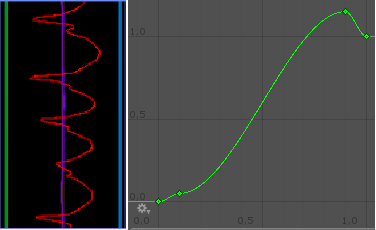
\includegraphics[width=.6\textwidth]{img/botMoveCurve.png}
  \caption{Horizontal bot movement (left) obtained when using the curve on the right}
  \label{fig:onemoveCurve}
\end{figure}


The movement made in a frame corresponds to the angle to be reached in that frame minus the angle reached in the previous frame. Finally, a point is determined in the initial interpolation variable where the bot will perform the click action (only in the case where it is aiming at a target it can destroy). Some noise can be added to each variable to simulate the inaccuracy of the bot.

In our trainings, we have used a curve that exceeds the upper limits, and in which the bot clicks on the highest end (See figure~\ref{fig:onemoveCurve}). This means that when aiming at small targets using long moves, the bot would overshoot the target and fire without hitting the opposite side of the one that started the move.

\subsection{``Cheat sheet'' rewards} %explicar como funciona el sistema de recompensas, incorporar SAC y PPO
\label{sec:cheatsheetD}

As we have seen in the section~\ref{sec:afterimpulse} with movement queues, not giving instant rewards but a time later can make it difficult to learn the neural network, plus it is more difficult to balance rewards in these cases where there is randomness in the exact moment an event occurs.

To solve these problems and at the same time accelerate the learning process we have designed the ``cheat sheet rewards''. These rewards are based on that the NPC itself is the one that determines the accuracy with which the agent has performed the action of clicking, and it does it before (or after) the NPC has performed it. The reward is calculated using a simple tolerable range (See~\ref{sec:tolrange}) by comparing the difference between the interpolation value in the frame the bot action is performed and the interpolation value at which the agent would perform the action.

Whenever the AI or the NPC performs a click action, an event is triggered. There are several factors to consider when using these rewards:
\begin{itemize}
	\item If the AI performs an action outside of the tolerable range (or when the agent is in idle~\footnote{Idle move corresponds to when the agent isn't seeking any target} move) is penalized
	\item An action performed inside the tolerable range is rewarded (the closest it is, the more the reward)
	\item Only the first action inside the tolerable range is rewarded, any other extra action is punished (not doing so would cause the agent to spam the click when it is close to the tolerable range)
	\item If the agent misses a click, the bot sends it a signal that causes it to receive a punish
\end{itemize}

This method can be used either with SAC or PPO, and with both algorithms correct results have been obtained: both the agent and the bot fail and hit certain targets in a similar way (although not always in the same cases). Nevertheless, there are still a few occasions in which the agent can perform the click action in some situations where it should not, without apparent reason (See Figure~\ref{fig:discCases}).

%imagen al final

\subsection{Discrete and continuous action spaces}
\label{sec:discVScont}
%diferencias en rendimiento, comportamiento, etc

When creating agents, Unity allows to use two action spaces: discrete and continuous~\footnote{Do not confuse action space with actions to be imitated (clicks in this case): as we will see later, discrete actions can be modeled using both continuous and discrete action space}. In discrete action spaces, there is a set of determined actions represented each one by an integer; in continuous action spaces, the action is represented with a float (this type of action is ideal for actions like mouse movement, which movement cannot be represented accurately using only integers).

However, ML Agents doesn't allow to combine both action spaces in one agent: all actions must be either discrete or continuous. If we wanted to create a neural network that could move and click by itself, its action space type would have to be continuous. Other option is to use two separate neural networks, one with all discrete actions and the other with the continuous ones. In this section this problem doesn't appear since we only want to imitate the clicking action, but still both methods have been tested.

To model discrete actions using continuous action space type, we consider the moment the action crosses the 0 line (when one action has negative action and the next positive value) as the moment when the agent triggers a click event. That can be consider as a mouse click, when the button is pressed a click event happens; but there cannot be another event until it is released (it returns to negative values). When using this method it is usually ideal to provide the agent the last action values as an observation, since it would tend to stay in positive values when being close to the target (if it fails to hit at first, the action has to return to negative values to perform another click).

To model discrete actions using discrete action space type, we have 2 actions: not clicking (0) and clicking (1). We can use the same method as with continuous action space (only the first consecutive ``1'' is considered as a click), or take every click action as an actual click. The second method is more reliable in practice, but produces more clicks that can cause the bot to receive very low rewards at first that can make the training session unstable.

In this test case, when using either SAC or PPO, continuous space type has better results (See figure~\ref{fig:discCases} to compare how both methods appear in the debug). Agents with discrete action spaces tend to perform much many pointless click (during idle movement) than agents with continuous space type, which usually have a 50-60\% success rate. However, since the environment was designed for continuous space actions, that can have caused that the agents with discrete action spaces perform worse than their continuous counterparts.

\begin{figure}[h]
  \centering
		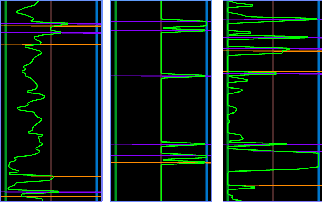
\includegraphics[width=.85\textwidth]{img/gphDiscActions.png}
  \caption{Discrete action agents: trained with SAC in continuous action space (left), with SAC but in discrete action space (mid) and with behavioral cloning in continuous action space (right). Orange lines correspond to the NPC clicks, and purple ones are click events triggered by the AI}
  \label{fig:discCases}
\end{figure}

\subsection{Models with behavioral cloning}%por que no funciona (ni gail)

Even though behavioral cloning is very effective with time noise (as seen in section~\ref{sec:timeBC}), it has a much harder time when imitating discrete actions. How well or badly it acts depends entirely on the demonstration~\footnote{In ML Agents, demonstrations are recorded using the actions provided in the heuristic function of the agent. These demonstrations are intended to be made by a human, but they can also be recorded from any NPC that can be accessed from the agent script} provided in the training session.

When using continuous action space, the action to be imitated is not just a boolean value, but a continuous number that meets the conditions to perform discrete actions described in section~\ref{sec:discVScont}. The easiest way is to assign a random value between -1 and 0 when the NPC is not performing a click, and a random value higher than 0 in the frame when it is clicking (demonstrations with uniform integer values perform worse). After less than 10000 steps, the neural network starts performing some clicks, but its performance is much worse than any model trained using SAC or PPO (see figure~\ref{fig:discCases}).

Problems that appear when using behavioral cloning in discrete action spaces are described in the following section.


\subsection{The frame problem}
%demonstration recorder y por que ocurre (flujo) (imagenes)

\begin{wrapfigure}{rH}{0.25\textwidth}
    \centering
    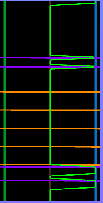
\includegraphics[width=0.2\textwidth]{img/bcStuck.png}
		\caption{NPC getting stuck because of the one frame problem}
		\label{fig:bcStuck}
\end{wrapfigure}

The one frame problem occurs in most demonstrations recorded for behavioral cloning (or GAIL), and it is caused because of how the information flows in each execution cycle in Unity.

As the game was built (See section~\ref{sec:sysarch}), the AI and the NPC are connected only through the Camera controller~\footnote{In latter trainings they were connected to create Cheat Sheet rewards, but the the heuristic function remained unchanged}. Then, the information flows in the following way: the NPC makes an action and it is sent in the first frame, the camera controller receives it (and actually performs it) in the second frame, and then the AI reads that action in frame 3. This delay of 1 frame between the action in the game and the action in the demonstration was negligible in continuous movements (mouse), however, in this case it causes the agent to learn to click when the target has been destroyed.

This problem is not very noticeable when training, but when using the neural network to perform the clicks it makes the NPC get stuck at pointing a target (In this section, the NPC is always the one controlling the movement). Only when the NPC recovers control of the action and destroys the target, the AI does perform. In figure~\ref{fig:bcStuck} you can see how the NPC gets stuck and clicks continuously when the AI is in control at the beginning (the first orange line corresponds to the first NPC click), and just after it recovers control in the click action (before the last orange line) and destroys the target, the AI performs a click action.

This problem can be solved by connecting the AI and the NPC so that it receives the information at the same time as the camera, but it is still outperformed by models trained with SAC and PPO in continuous action spaces.

\section{Complex movements}

In this section we try to create an agent that imitates a more complex movement. To do so, we have used the bot described in section~\ref{sec:botshaped}, but with curves that have different shapes (see Figure~\ref{fig:compCurve}). In the following training sessions we won't take into account the click actions to avoid interferences in the rewards. In this case, the bot always clicks at an interpolation value of 1, so it always destroys the target at the same time that a movement ends.

\begin{figure}[h]
  \centering
		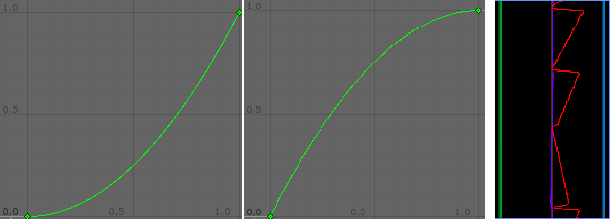
\includegraphics[width=.8\textwidth]{img/gphCompActions.png}
  \caption{Movement curves for seeking target (left) and idle (mid). The right picture shows the bot's movement with one seek target in the middle (purple line is vertical move and red line is horizontal move, both have the same shape).}
  \label{fig:compCurve}
\end{figure}

\subsection{Debug for 2 axis} %describir un poco el debug (+imagen)

The graphics used so far are no longer completely effective in 2-axis movements: even if the bot can do one of the 2 axis well, if it did the other one wrongly, the movement obtained would be very different from that of the NPC to be imitated.

\begin{figure}[h]
  \centering
		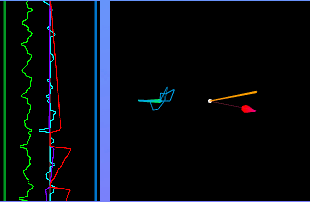
\includegraphics[width=.8\textwidth]{img/debug2axis.png}
  \caption{Shaped movement of the bot (red-purple lines) and a continuous movement to the left from one agent (green-blue lines) in both of the debug graphics}
  \label{fig:debug2axis}
\end{figure}

In this kind of movements, when following targets the direction the bot takes (and the speed in some sense) is more important than the X and Y components treated independently. For this reason, the following graph has been created to debug the bots, showing the direction and speed in each frame. The values shown on it could be compared to the functioning of a joystick: the movement is in the direction of the point with respect to the origin, and the further from the center it is the faster it will move (See Figure~\ref{fig:debug2axis}).

This graph, in addition to the previous one, allows a better understanding of the progress of a bot during training and helps to find problems to correct.

\subsection{Angle-Magnitude reward system} %empezar con TR y describir AM

The first reward system devised for the task developed in this section was the tolerable range, but instead of applying it to the difference between each movement it is applied to the distance in the plane between the points (X, Y) of the NPC and the AI movements. As we can see in figure~\ref{fig:axisTR}, in the line graph the movements seem to adapt to the shape (at least in the horizontal ones, which correspond to those of greater magnitude), but in the plane graph we can see that the movement is much more chaotic than it seemed (especially due to the noise in the vertical movements).

\begin{figure}[h]
  \centering
		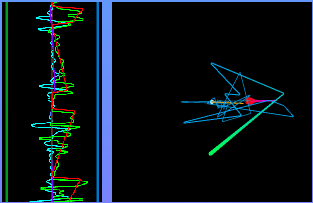
\includegraphics[width=.8\textwidth]{img/axisTR.png}
  \caption{Agent trained with tolerable range, shown in both debug graphs}
  \label{fig:axisTR}
\end{figure}

In order to achieve a reward system that is easier to balance and allows to get agents with less noise, a method has been designed to create rewards using angle and magnitude as parameters. In this way, more weight can be given to one of the 2 parameters depending on what is intended to be achieved in the agent (or to adjust the rewards to obtain better results). In Figure~\ref{fig:axisTR} you can see an example of an agent resulting from a training with angle-magnitude tolerable range: the AI adapts to the shape of the movement and follows the same angle although with still too much noise (in the first frame of a new idle movement it usually does not have much precision, since it is determined randomly).

\begin{figure}[h]
  \centering
		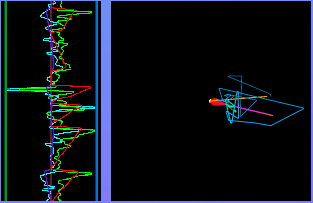
\includegraphics[width=.8\textwidth]{img/axisAMTR.png}
  \caption{Agent trained with angle-magnitude tolerable range}
  \label{fig:axisAMTR}
\end{figure}

\subsection{Cheat sheet for movements} %regresion lineal, y como funciona este metodo

The main problem that appears when using tolerable range is that it scores or penalizes all movements equally, which causes it to: have very significant errors at the beginning (when the movement is not predictable), adapt more or less well in the center, and then in the final frames it makes errors again (in this case, because the neural network has more difficulty in matching movements that are very small in magnitude, and the range allows it to go further than it should despite being predictable). In addition, in vertical movements the agent usually has an excess of noise because its magnitude is much lower than that of the horizontal ones (a solution to this problem is proposed in section~\ref{sec:improving}).

Weighing the penalties correctly using a traditional reward system may involve taking into account parameters such as the coherence of the movement as  previously seen, but applied to a linear regression~\footnote{A linear regresion would make sense for the particular movement we are dealing with in this section, as it can be shaped with straight lines. However, these methods would be too dependent on the concrete form of the movement and very difficult to generalize} that allows to predict the next movement, and modifying the weight of the rewards and penalties at each point in the movement to give more exigency in points where the movement is predictable and less where it is almost random.

To achieve a similar and easy to modify effect, we have created a ``cheat sheet'' shaped reward system (Section~\ref{sec:cheatsheetD}) in which you can change the value of the punishment and reward parameters at each point of the interpolation of a movement by means of curves. To speed up the process and simplify the task, the movement of chasing a target is not taken into account, so it has been possible to eliminate the camera (the agent only receives information about the movement it is doing). In the Figure~\ref{fig:axisCS} you can see the curves that have been used in the most successful trainings.

\begin{figure}[h]
  \centering
		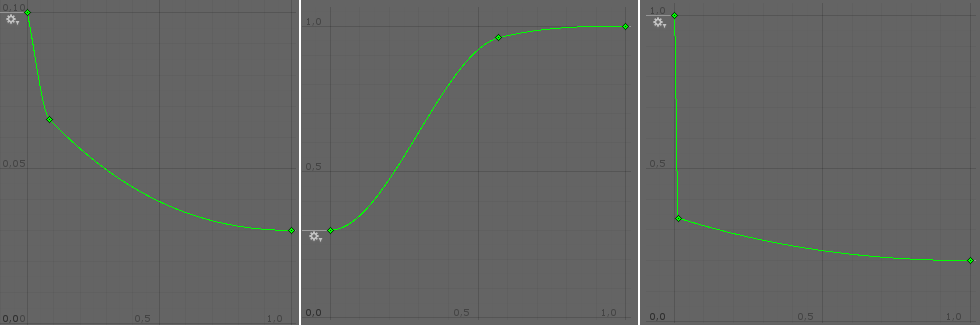
\includegraphics[width=1\textwidth]{img/axisCS.png}
  \caption{Curves for tolerable range (left), punish factor (mid) and reward factor (right)}
  \label{fig:axisCS}
\end{figure}

In figure~\ref{fig:axisbestCS} you can see one of the models that best adapts to the NPC's movement: it is noticeable that the bot still has some noise and still doesn't perform very well in the beginning and at the end of the movements, but it tends to stay near the angle of the original move. However, in this case we didn't take into account the seeking cases and it only uses observations of the NPC movement, so this agent would not be able to play the game independently.

\begin{figure}[h]
  \centering
		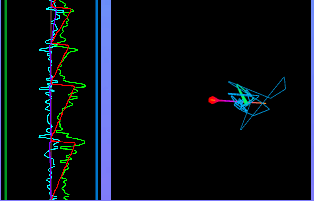
\includegraphics[width=.6\textwidth]{img/axisBestCS.png}
  \caption{Agent trained with shaped rewards}
  \label{fig:axisbestCS}
\end{figure}

\subsection{Movement interdependency} %problema al ejecutar el bot solo (hablar tambien de observaciones de bot vs agente) (+imagen con el mejor resultado y una grafica plana)

In practically all the agents developed in this section, it has been used as observations the previous movements made by the NPC, instead of those made by the agent. 

\begin{figure}[h]
  \centering
		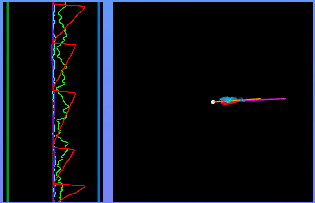
\includegraphics[width=.6\textwidth]{img/axisInterdep.png}
  \caption{Agent trained using its own observations}
  \label{fig:axisInterdep}
\end{figure}

The problem that presents the interdependence of movements is that in the training the agent learns from the movements generated by the bot, so it is easier to predict the next one. Once the agent plays by himself, it must not only perform movements but also use its previous movements as observations for the next ones. In cases where the agent has too much noise in its moves, this can cause it to end up getting stuck or making meaningless moves.

In some of the cases of this section, using observations of the agent (both in full training and at the end) causes them to move in the correct direction but with constant magnitude (See Figure~\ref{fig:axisInterdep}). Other agents that have been trained using only observations of the bot can move very chaotically

Ideally, for a workout to be correct enough, it should end up showing correct behavior while receiving as observations its own movements rather than those of the bot. In a perfect training, the agent would end up controlling the movement of the game (and performing it in a similar way to the NPC). However, none of these 2 conditions could be achieved in this section.

\subsection{Trying to improve performance}
\label{sec:improving} %sensibilidad, AM action space (subsubsections), quitar rt

In this subsection, several experiments that were attempted to correct certain errors that appeared when training agents from this section are presented.

\subsubsection{Mouse sensitivity}

\begin{figure}[h]
  \centering
		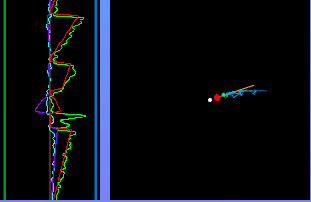
\includegraphics[width=.6\textwidth]{img/axisYsens.png}
  \caption{Agent with Y sensitivity of 10}
  \label{fig:axisYsens}
\end{figure}

The sensitivity of the mouse was intended to give the bot more precision in vertical (Y axis) movements (which are usually much smaller in magnitude than horizontal ones). This was achieved by dividing the action of the neural network by a value. Although it improved the accuracy in most cases, the network was practically prevented from making minimally fast vertical movements (for example, when a target appears above). Figure~\ref{fig:axisYsens} shows an example of agent that was trained using a sensitivity of 10: in the line graph it can be seen that the agent adapts very well to almost all movements with precision, except when the vertical movement is slightly larger; in the plane graph it is also visible that the agent doesn't reach the higher vertical moves (the line is slightly curved).

\subsubsection{Momentum}

When using the reward curves shown in Figure~\ref{fig:axisCS}, the agents usually ``anticipated'' the next move instead of ending the current move well (see Figure~\ref{fig:axisMomentum}). This was because the first frame of a move offered a much higher and easier reward than the last. \emph{Momentum} is a variable that oscillates between -0.75 and 0.75: starting at 0, when the agent receives a positive reward, the momentum is increased by 0.125, if it receives a negative reward, it is decreased. For example, a momentum of 0.75 causes positive rewards to be multiplied by 1.75, and negative rewards by 0.25 (and the opposite happens with negative momentum). Then, if the agent fails some consecutive actions in the last frames of a movement, the punishments are increased stepwise and the reward obtained in the first frame of the next movement is reduced considerably (depending on how many consecutive actions the agent has failed before).

\begin{figure}[h]
  \centering
		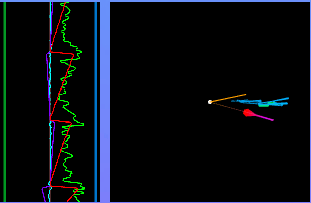
\includegraphics[width=.6\textwidth]{img/axisMomentum.png}
  \caption{Agent that tends to anticipate next movements}
  \label{fig:axisMomentum}
\end{figure}

The effectiveness of this parameter is difficult to be appreciated, however, the best results obtained in this section were trained using momentum.

\subsubsection{Angle-Magnitude actions}

It also was tried to create a bot that performed actions based on angle and magnitude (direction and velocity), instead of X movement and Y movement. It was tested using previous X and Y movements as observations, and previous angles and magnitudes.

\begin{figure}[h]
  \centering
		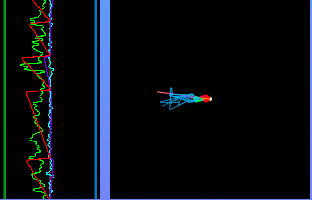
\includegraphics[width=.6\textwidth]{img/axisAMact.png}
  \caption{Agent with angle-magnitude actions (the bot was reversed to avoid crossing the 0-line)}
  \label{fig:axisAMAS}
\end{figure}

In theory, imitating the bot with the information presented in this way should have been trivial for the agent (the angle remains constant throughout the movement, and the magnitude decreases linearly to 0), but the results obtained were not very different from those using the X and Y movements as action and observation, they were even worse (See Figure~\ref{fig:axisAMAS}). Also, it had difficulties to follow the bot's movement when the angle changed crossed the 0 degree line (an angle of 0 degrees corresponded to an action of -1, and an angle of 360 to +1).

%conclusiones (en el fichero 5)